كما أشرنا سابقاً فإنّ عمليّة التّحكم مركزيّة؛ حيث يوجد نظام تشغيل ROS على الحاسوب المركزي. يوجد على نظام ROS ثلاث عقد أساسيّة.
العقدة الأولى : تتصل مع الكاميرا المثبّتة أعلى المنصّة، حيث تقوم الكاميرا بإرسال الأطر لها لتقوم باستخلاص معلومات عن الخريطة ومواقع الرّوبوتات. ولتحقيق القراءة الدقيقة لمواقع الروبوتات في الزمن الحقيقي على الحاسوب المركزي سنعتمد مكتبة ArUco وهي مكتبة تستخدم في تطبيقات الواقع المعزز وتعتمد على مكتبة OpenCV  وتساعد في عملية معايرة الكاميرا. سيتم تثبيت علامات QR-markers على الروبوتات ومنه تقوم عقدة ال ArUCo في ال ROS تقوم باكتشاف وتحديد موقع العلامات وترسلها لل ROS-TOPIC .



\begin{figure}
	\centering
	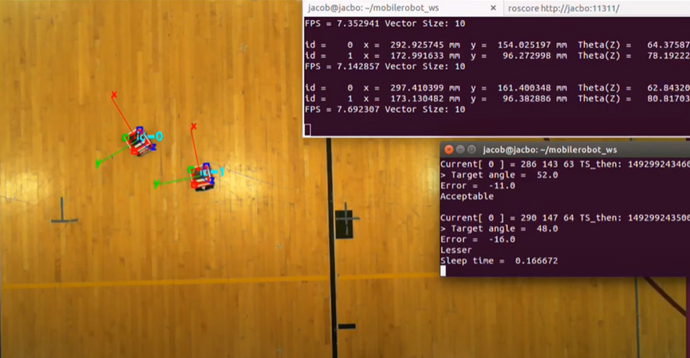
\includegraphics[width=0.7\linewidth]{figs/20/fig20_1}
	\caption{صورة توضيحيّة لآليّة عمل محددات ArUco}
	\label{20:fig:1}
\end{figure}

العقدة الثّانية: تقوم هذه العقدة باستقبال إحداثيّات الرّوبوتات والعوائق من العقدة الأولى عن طريق اشتراكها بالـ ROS TOPIC ذاته. بعد ذلك تتمّ على هذه العقدة عمليّة توليد المسار الأمثل وفق الخوارزميّة المختارة وإرسال نقاط المسارات الكاملة لجميع الرّوبوتات إلى العقدة الثّالقة.
العقدة الثّالثة: بعد استقبال هذه العقدة لنقاط المسارات الكاملة لجميع الرّوبوتات، تقوم بإرسال كلّ مسار إلى الـ Topic الخاص به  (إلى الرّوبوت الخاص به المشترك بنفس الـ Topic) عن طريق مخدّم الـ mqtt، لتكون هذه العقدة يمثابة عقدة وصل بين نظام ROS و مخدّم بروتوكول الـ mqtt.
وبعد أن يستقبل كلّ روبوت الرّسائل الخاصّة به تتكرّر هذه العمليّة بشكل دوري، ثمّ يقوم كلّ روبوت بتتيّع المسار وفق خوارزميّة تصحيح PID.
